\section{Preliminary Results}
\label{sec:results}

\noindent\textbf{Dataset and setup.}
We report a reproducible pilot on a balanced $N{=}20$ subset of SPECS,
drawn from the 400-image five-city pool available locally in this
release (80 images each from Amsterdam, Abuja, San Francisco,
Santiago, and Singapore). We sample 4 images per city using the same
vision-based stratification described in Section~\ref{sec:method}:
baseline safety score together with visual complexity. For each scene we
allow up to $K{=}3$ lever candidates and a bounded stochastic budget of
$T{=}1$ generation attempt per fixed candidate lever. The resulting run
is fully reproducible from the released scripts and configuration.

\begin{table}[t]
  \centering
  \caption{Actual pilot setup and aggregate outcomes for the reproducible
  $N{=}20$ run.}
  \label{tab:setup}
  \small
  \begin{tabular}{p{0.54\linewidth}p{0.22\linewidth}}
    \toprule
    Setting & Value \\
    \midrule
    Source pool & 400 SPECS scenes (5 cities, 80 each) \\
    Pilot subset & $N{=}20$ (4 per city) \\
    Sampling & Per-city safety score + complexity stratification \\
    Attribute & Safety (increase direction) \\
    Candidate budget $K$ & 3 per image \\
    Stochastic budget $T$ & 1 per lever \\
    Generator & \texttt{flux-kontext-max} \\
    Auxiliary scorer & ViT-PP2 safety classifier \\
    Realized candidate rows & 38 \\
    Valid edits & 13 / 38 (34.2\%) \\
    Mean valid-edit coverage & 0.217 \\
    \bottomrule
  \end{tabular}
\end{table}

\noindent\textbf{Validity and coverage.}
The dominant bottleneck in the current pipeline is not candidate
proposal but valid realization. Across 20 scenes, the planner produced
38 candidate rows in total (1.9 candidates per image on average after
ontology filtering), of which 13 passed the validity audit. This yields
mean coverage of $|V(x)|/|L(x)| = 0.217$. Only 8 of 20 scenes admit at
least one valid realized intervention, and only 3 of 20 scenes admit
more than one. Figure~\ref{fig:distribution} shows the full
distribution: 12 scenes have zero valid realized levers, 5 have one, 1
has two, and 2 have three.

\begin{table}[t]
  \centering
  \caption{Failure analysis for the reproducible $N{=}20$ pilot.
  The first row is a pre-audit generator failure count. Audit rows are
  computed over the 14 audited but invalid edits and are non-exclusive.}
  \label{tab:failure}
  \small
  \begin{tabular}{p{0.54\linewidth}p{0.22\linewidth}}
    \toprule
    Failure mode & Count \\
    \midrule
    Generator failure before audit & 11 \\
    Implausible intervention & 12 / 14 \\
    Non-local drift & 8 / 14 \\
    Unrealistic rendering & 1 / 14 \\
    Same-place failure & 0 / 14 \\
    \bottomrule
  \end{tabular}
\end{table}

This breakdown clarifies where the pipeline currently fails. The first
loss point is generator reliability itself: 11 rows in this run never
reached a usable audited edit. Among the edits that were audited but
rejected, plausibility and locality dominate, whereas same-place
preservation is not the main problem. In other words, the system more
often keeps the street identity but fails to make a convincing,
localized version of the requested lever.

\begin{figure}[t]
  \centering
  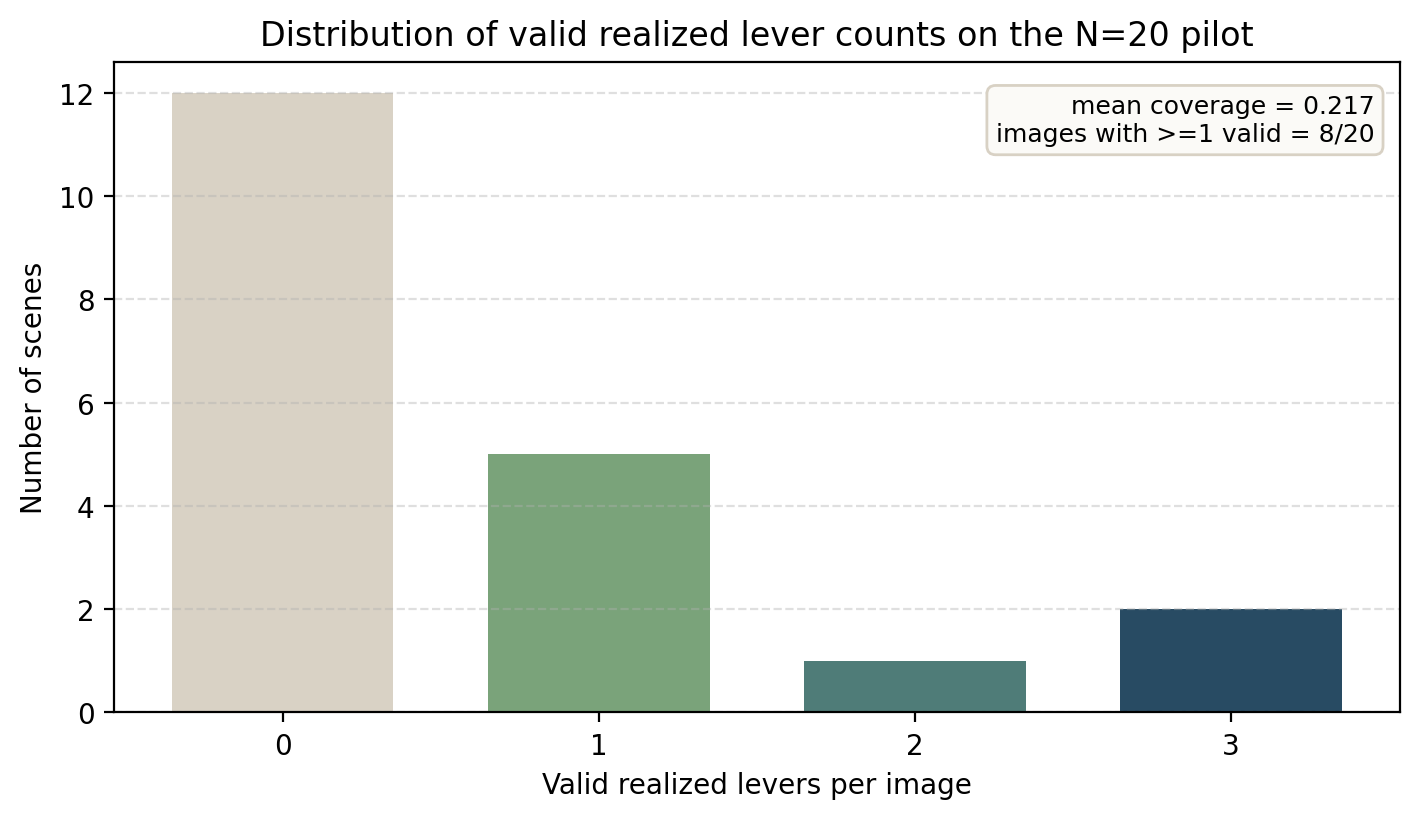
\includegraphics[width=\columnwidth]{figures/figure_2_valid_distribution.png}
  \caption{
    Distribution of valid realized lever counts on the reproducible
    $N{=}20$ pilot. Most scenes still yield no valid accepted edit under
    the current prompt-only pipeline, indicating that realization
    reliability remains the main limiting factor.
  }
  \label{fig:distribution}
\end{figure}

\noindent\textbf{Auxiliary directional shifts.}
Among the 13 valid edits, the auxiliary classifier produces a mean
directional shift of $+0.723$ (median $+0.451$, max $+3.525$, min
$-0.974$). Using the exploratory auxiliary threshold
$\theta_{\mathrm{aux}}{=}0.1$, 9 of 13 valid edits exceed threshold.
These values should be interpreted only as pilot ranking signals, not
as human-grounded effectiveness estimates. The strongest positive shifts
in this run come from localized litter removal, lane marking repainting,
crosswalk repainting, and modest frontage cleanup/greening. Notably,
some edits that are clearly valid still produce negative auxiliary
movement, which reinforces the need to separate realization success from
perceived attribute improvement.

\begin{table}[t]
  \centering
  \caption{Observed pilot metrics from the reproducible $N{=}20$ run.}
  \label{tab:main}
  \small
  \begin{tabular}{p{0.54\linewidth}p{0.22\linewidth}}
    \toprule
    Metric & Value \\
    \midrule
    Images with any valid edit & 8 / 20 \\
    Images with $>1$ valid edit & 3 / 20 \\
    Mean valid levers per image & 0.65 \\
    Valid-count histogram & 12 / 5 / 1 / 2 for 0 / 1 / 2 / 3 \\
    Mean auxiliary delta & +0.723 \\
    Median auxiliary delta & +0.451 \\
    Max auxiliary delta & +3.525 \\
    Valid edits above $\theta_{\mathrm{aux}}$ & 9 / 13 \\
    \bottomrule
  \end{tabular}
\end{table}

\begin{table}[t]
  \centering
  \caption{Lever-type breakdown over audited candidate rows with
  non-empty lever identities. Mean auxiliary delta is computed only over
  valid rows for that lever type.}
  \label{tab:levers}
  \scriptsize
  \begin{tabular}{p{0.48\linewidth}ccc}
    \toprule
    Lever concept & Proposed & Valid & Mean $\Delta_{\mathrm{aux}}$ \\
    \midrule
    Surface cleaning & 7 & 3 & 0.084 \\
    Tree canopy management & 5 & 1 & -0.106 \\
    Lane marking repainting & 4 & 3 & 0.906 \\
    Lighting repair & 4 & 0 & -- \\
    Litter removal & 3 & 2 & 1.893 \\
    Crosswalk repainting & 2 & 2 & 0.805 \\
    Localized greenery addition & 2 & 2 & 0.569 \\
    \bottomrule
  \end{tabular}
\end{table}

Table~\ref{tab:levers} shows that the current pipeline is materially
better at some lever families than others. Repainting and cleanup
interventions are both easier to realize validly and more likely to
produce positive auxiliary shifts, whereas lighting repair and tree
canopy management remain difficult under prompt-only editing. This is a
useful workshop result even without human evaluation: the protocol does
not merely rank scenes, it exposes which classes of localized urban
counterfactual are currently operational.

\noindent\textbf{Qualitative examples.}
Figure~\ref{fig:qualitative} shows the top three positive auxiliary-shift
examples from distinct scenes in the pilot. They are representative of
the types of interventions that currently survive the validity audit:
localized cleanup, lane-marking repainting, and crosswalk repainting.
All three are spatially constrained, visually legible, and plausible as
single-lever urban changes. At the same time, they also illustrate the
current framing of the paper: these are \emph{valid and directionally
promising} interventions under an auxiliary scorer, not finalized human
effect estimates.

\begin{figure}[t]
  \centering
  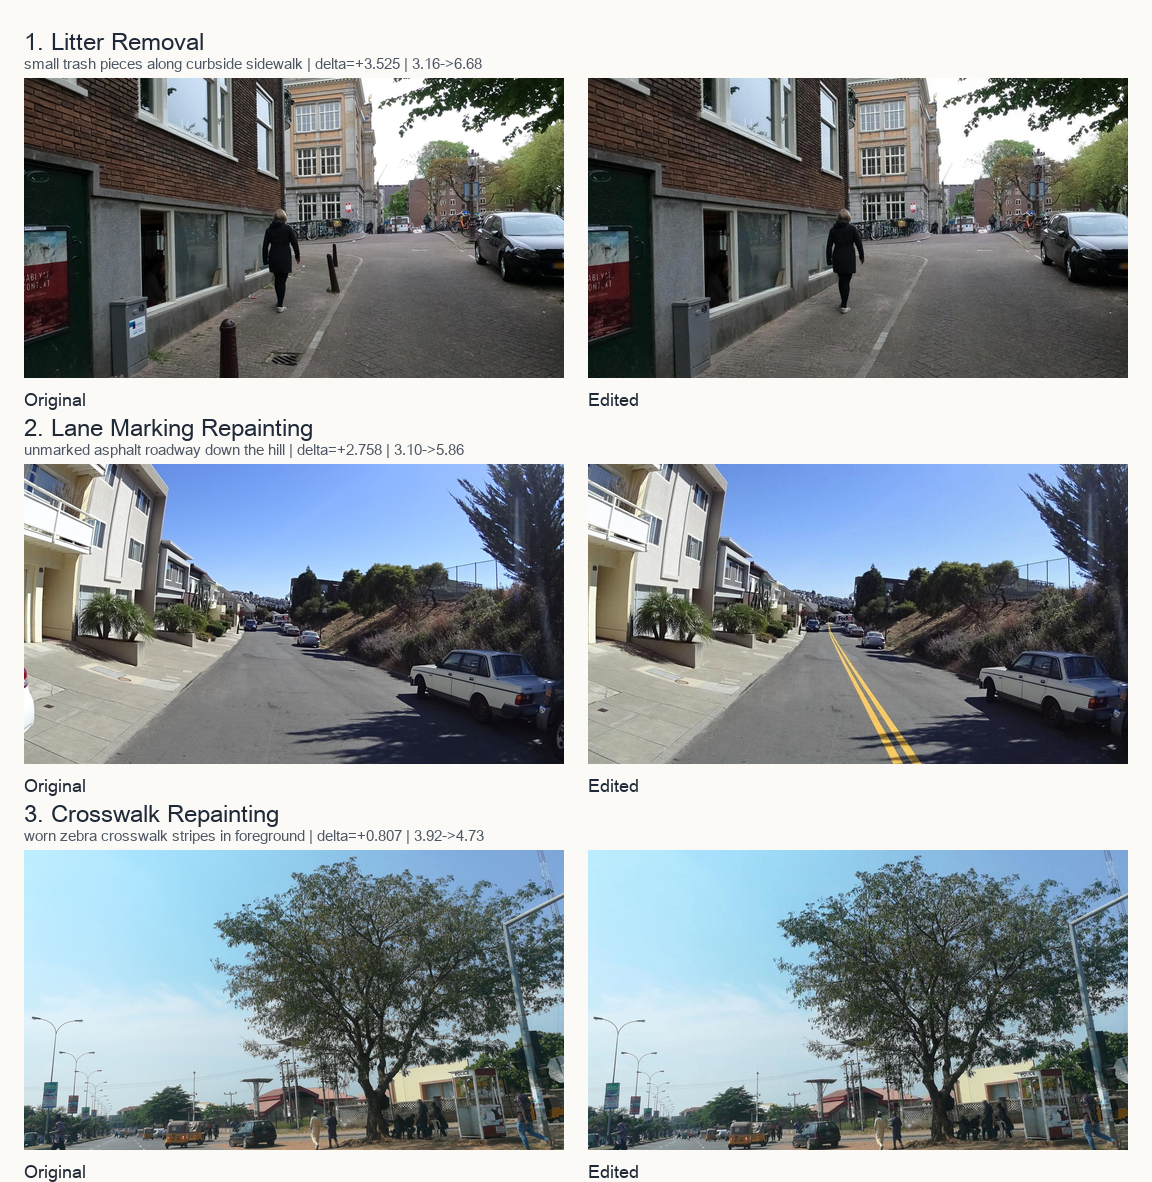
\includegraphics[width=\columnwidth]{figures/figure_3_qualitative.png}
  \caption{
    Top three distinct-scene qualitative examples ranked by auxiliary
    classifier delta in the $N{=}20$ pilot. From top to bottom: litter
    removal, lane-marking repainting, and crosswalk repainting. These
    examples illustrate the interventions that the current pipeline can
    realize validly; they do not by themselves establish human-perceived
    effectiveness.
  }
  \label{fig:qualitative}
\end{figure}
